\subsection{Proxy (\textit{o Surrogate})}
\label{proxy}

\textbf{Scopo}: Strutturale \\
\textbf{Raggio d'azione}: Oggetti

\paragraph{Definizione} Fornisce un surrogato o segnaposto di un altro oggetto per controllare l'accesso a tale oggetto.

\paragraph{Motivazione} Si consideri un editor che consente di rappresentare anche immagini all’interno dei documenti. Per velocizzare il caricamento in memoria dei documenti può essere opportuno ritardare il caricamento delle immagini fino a quando non è necessario visualizzarle.

\begin{figure}[H]
    \centering
    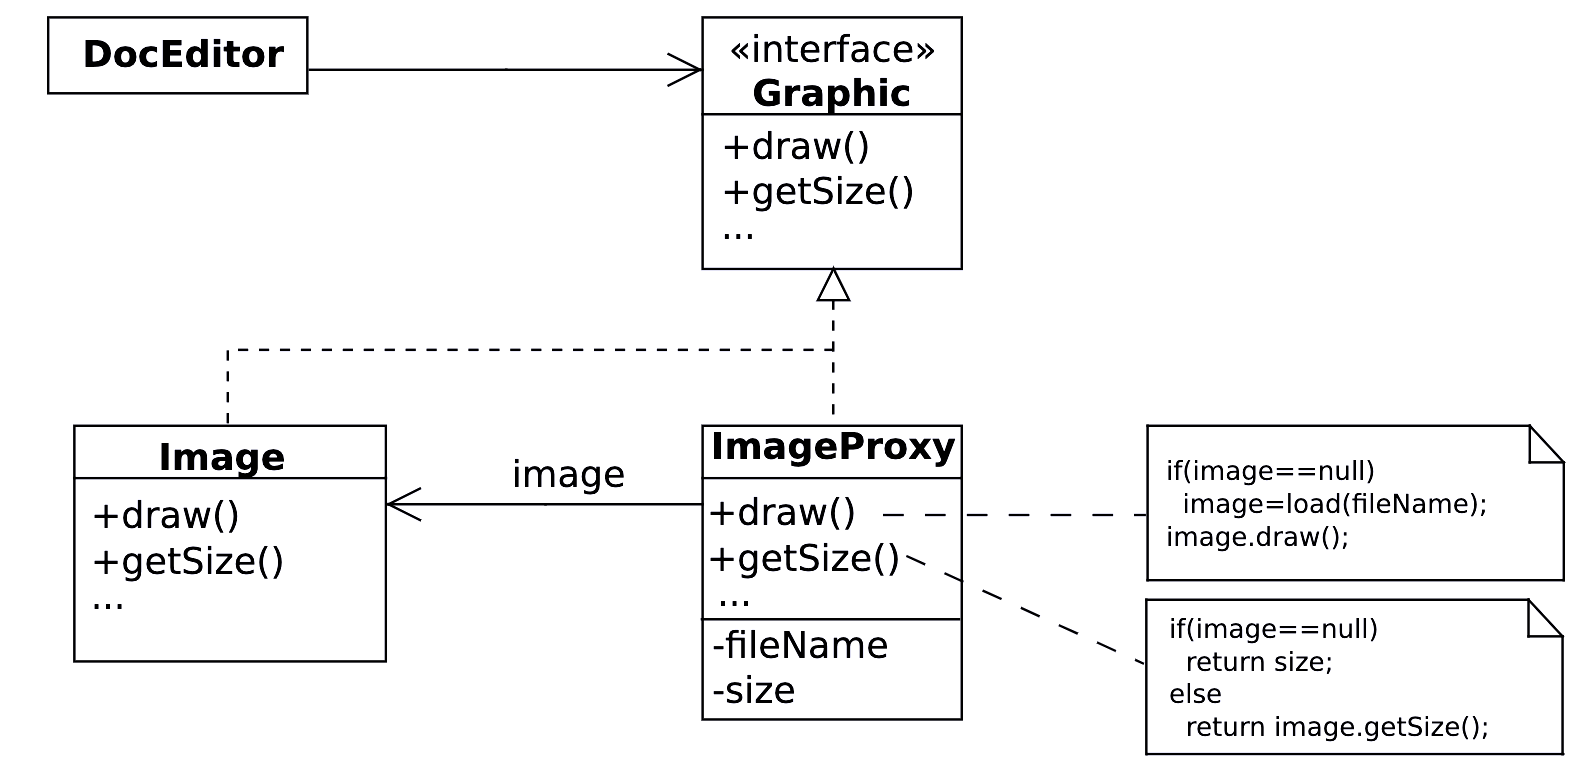
\includegraphics[width=0.75\linewidth]{assets/pattern/proxy/proxy-esempio.png}
    \caption{Esempio di utilizzo del pattern}
\end{figure}

La soluzione consiste nell'utilizzare un oggetto surrogato dell’immagine, ad esempio che pre-occupi lo stesso spazio.

\paragraph{Applicabilità} Il pattern Proxy è utilizzabile nelle seguenti situazioni:
\begin{itemize}
    \item \textbf{Remote Proxy}: fornisce una rappresentazione di un oggetto in un diverso address-space;
    \item \textbf{Virtual Proxy}: crea oggetti costosi su richiesta;
    \item \textbf{Protection Proxy}: controlla l'accesso all'oggetto originale;
    \item \textbf{Smart Reference}: è un sostituito di un puntatore classico che esegue ulteriori operazioni quando un oggetto viene utilizzato;
\end{itemize}

\paragraph{Struttura} Il pattern è composto da:
\begin{itemize}
    \item \textbf{Proxy} (ImageProxy): mantiene un riferimento all'oggetto di tipo RealSubject (di cui è \textit{surrogato}). Ha la stessa interfaccia di Subject. Controlla l'accesso all'oggetto rappresentato e può essere responsabile della sua creazione o eliminazione;
    \item \textbf{Subject} (Graphic): definisce l'interfaccia comune per RealSubject e Proxy consentendo di usare Proxy ove ci si attende un RealSubject
    \item \textbf{RealSubject} (Image): definisce l'oggetto reale rappresentato dal proxy;
\end{itemize}

Il Proxy rimanda le richieste al RealSubject (se appropriato), in base al tipo di proxy.

\begin{figure}[H]
    \centering
    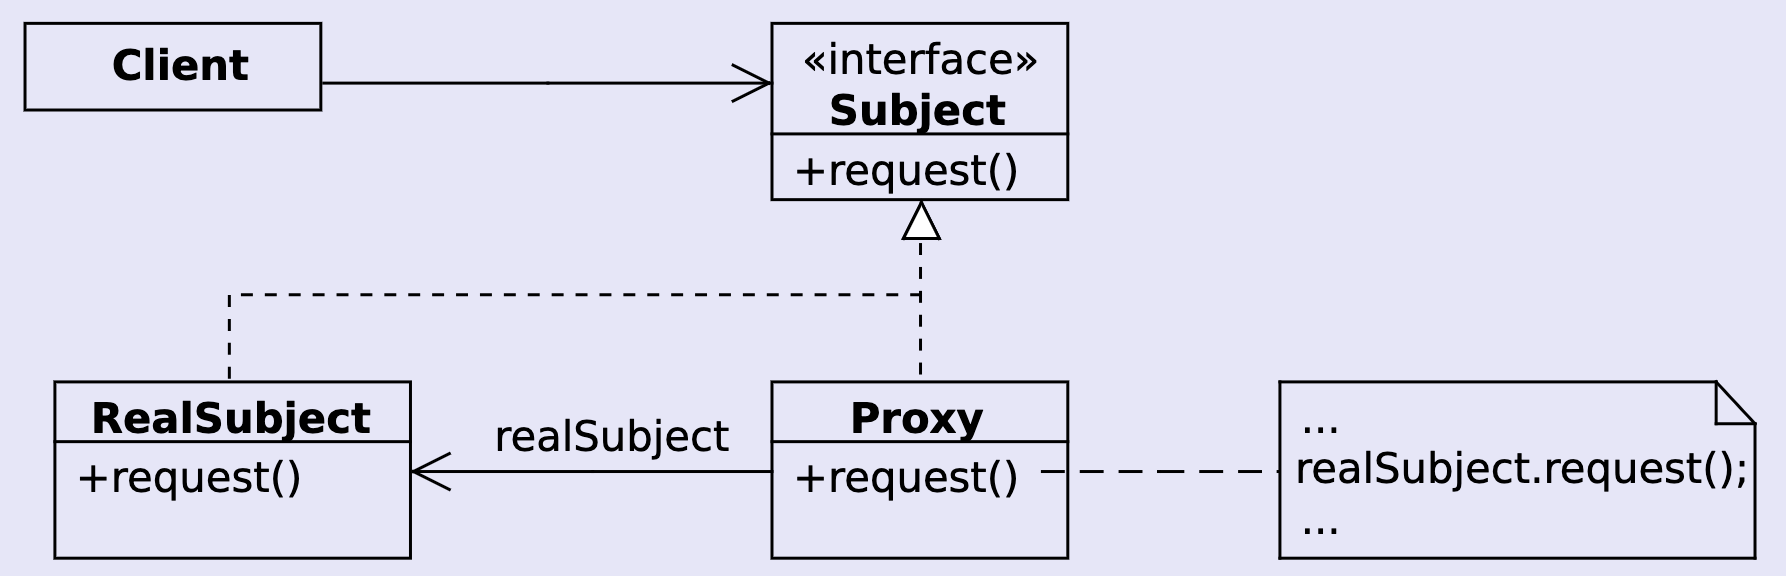
\includegraphics[width=0.75\linewidth]{assets/pattern/proxy/proxy-struttura.png}
    \caption{Class Diagram del pattern Proxy}
\end{figure}

\begin{figure}[H]
    \centering
    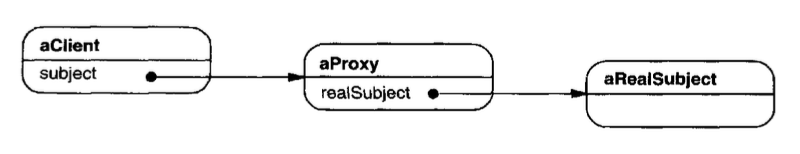
\includegraphics[width=0.75\linewidth]{assets/pattern/proxy/proxy-object-diagram.png}
    \caption{Object Diagram del pattern Proxy}
\end{figure}

\paragraph{Conseguenze} Il pattern Proxy consente quindi di:
\begin{itemize}
    \item Introdurre un livello di indirezione quando si accede ad un oggetto;
    \item Introdurre il \textbf{copy-on-write}: postporre il processo di copia fin quando l'oggetto non viene modificato.
\end{itemize}

\textbf{Esempio Java}
\begin{minted}[
    fontsize=\footnotesize,
    linenos,
]{java}
// Proxy implements Subject
public class ListaSicura<E> implements Lista<E> {

    private Lista<E> lista;
    private PermessiUtente pu; // RealSubject

    public ListaSicura(Lista<E> l, int nread, int nwrite) {
        lista = l;
        pu = new PermessiUtente(nread, nwrite);
    }

    @Override
    public void aggiungi(int index, E dato) throws IndexOutOfBoundsException {
        if(pu.getNumeroScritture() == 0) {
            throw new AccessoNonConsentitoException
        }
        pu.decrementaScritture();
        lista.aggiungi(index, dato);
    }

}
\end{minted}


\newpage